\documentclass[aspectratio=169, lualatex, handout]{beamer}
\makeatletter\def\input@path{{theme/}}\makeatother\usetheme{cipher}

\title{Applied Cryptography}
\author{Nadim Kobeissi}
\institute{American University of Beirut}
\instituteimage{images/aub_white.png}
\date{\today}
\coversubtitle{CMPS 297AD/396AI\\Fall 2025}
\coverpartname{Part 2: Real-World Cryptography}
\covertopicname{2.6: Cryptocurrency Cryptography}
\coverwebsite{https://appliedcryptography.page}

\begin{document}
\begin{frame}[plain]
	\titlepage
\end{frame}

% Bitcoin (explain primitives here)?
% Ethereum and smart contracts
% L1 vs L2
% Zcash
% Penumbra

\begin{frame}{Slides not complete and may contain errors}
	\begin{itemize}
		\item This slide deck is not finished, may contain errors, and is missing important material. Do not rely on it yet.
	\end{itemize}
\end{frame}

\section{Bitcoin: The Designer's Perspective}

\begin{frame}{The problem: trust in digital commerce}
	\begin{itemize}
		\item Online commerce relies entirely on financial institutions as trusted third parties.
		\item Banks, payment processors, credit card companies mediate every transaction.
		\item This trust-based model has fundamental limitations:
		      \begin{itemize}
			      \item Intrinsic dependence on centralized parties.
			      \item Financial institutions must mediate disputes.
			      \item Increases transaction costs significantly.
		      \end{itemize}
	\end{itemize}
\end{frame}

\begin{frame}{Weaknesses of the trust-based model}
	\begin{itemize}
		\item \textbf{High transaction costs}: Mediation costs make micropayments impractical.
		\item \textbf{Reversibility spreads distrust}: Merchants need extensive customer information.
		\item \textbf{Fraud is inevitable}: Some percentage of fraud accepted as cost of business.
		\item \textbf{No digital cash equivalent}: Physical cash works person-to-person, but no digital. analog exists
	\end{itemize}
\end{frame}

\begin{frame}{Peer-to-peer electronic cash}
	\begin{itemize}
		\item Replace trust with cryptographic proof.
		\item Enable direct transactions between parties without intermediaries.
		\item Key properties needed:
		      \begin{itemize}
			      \item Computationally impractical to reverse (protects sellers).
			      \item Optional escrow mechanisms (protects buyers).
			      \item No reliance on third parties.
		      \end{itemize}
	\end{itemize}
\end{frame}

\begin{frame}{Core challenge: double spending}
	\begin{itemize}
		\item Digital information can be copied perfectly.
		\item Without a central authority, how do we prevent spending the same coin twice?
		\item Traditional solution: Central mint/bank tracks all transactions.
		\item Problem: This reintroduces the trusted third party.
	\end{itemize}
\end{frame}

\begin{frame}{Bitcoin's solution}
	\begin{itemize}
		\item Peer-to-peer distributed timestamp server.
		\item Generates computational proof of transaction order.
		\item Security assumption: Honest nodes control majority of CPU power.
		\item Key innovations:
		      \begin{itemize}
			      \item Proof-of-work consensus mechanism.
			      \item Blockchain as public ledger.
			      \item Economic incentives for honest behavior.
		      \end{itemize}
	\end{itemize}
\end{frame}

\begin{frame}{Historical context}
	\begin{itemize}
		\item Published October 31, 2008 by Satoshi Nakamoto (pseudonym)
		\item Built on decades of cryptographic research:
		      \begin{itemize}
			      \item Digital signatures (Diffie-Hellman, RSA)
			      \item Hashcash proof-of-work (Adam Back, 1997)
			      \item Cryptographic timestamps (Haber \& Stornetta, 1991)
			      \item B-money and bit gold proposals (Wei Dai, Nick Szabo)
		      \end{itemize}
		\item First practical solution to Byzantine Generals Problem for money.
	\end{itemize}
\end{frame}

\begin{frame}{The Byzantine Generals Problem}
	\begin{itemize}
		\item Classical problem in distributed computing (Lamport, Shostak, Pease, 1982).
		\item Scenario: Byzantine generals must coordinate attack on a city.
		      \begin{itemize}
			      \item Generals can only communicate via messengers.
			      \item Some generals may be traitors sending false messages.
			      \item Need consensus: all loyal generals execute same plan.
		      \end{itemize}
		\item Core challenge: How to achieve reliable consensus when:
		      \begin{itemize}
			      \item Communication channels are unreliable.
			      \item Some participants may be malicious.
			      \item No central authority to trust.
		      \end{itemize}
		\item \textbf{Bitcoin's breakthrough}: First practical solution for digital money using proof-of-work.
	\end{itemize}
\end{frame}

\subsection{Coins as digital signature chains}

\begin{frame}{Electronic coins as digital signatures}
	\begin{itemize}
		\item Bitcoin defines an electronic coin as a chain of digital signatures.
		\item Each owner transfers the coin by:
		      \begin{itemize}
			      \item Digitally signing a hash of the previous transaction.
			      \item Adding the next owner's public key.
			      \item Appending this to the end of the coin.
		      \end{itemize}
		\item The payee can verify ownership by checking the chain of signatures.
	\end{itemize}
\end{frame}

\begin{frame}{Transaction structure}
	\begin{itemize}
		\item \textbf{Transaction inputs}: References to previous transactions.
		\item \textbf{Transaction outputs}: Amount and recipient's public key hash.
		\item \textbf{Digital signature}: Proves the owner authorized the transfer.
		\item Coins don't exist as discrete units, only as transaction chains.
	\end{itemize}
\end{frame}

\begin{frame}{A coin is the set of its transactions}
	\bigimagewithcaption{bitcoin_transactions.png}{Source: Satoshi Nakamoto}
\end{frame}

\begin{frame}{How are coins created?}
	\begin{columns}[c]
		\begin{column}{1\textwidth}
			\begin{itemize}
				\item New coins are created through \textbf{mining} - the process of adding blocks to the blockchain.
				\item Each block contains a special \textbf{coinbase transaction}\footnote{Not to be confused with Coinbase, the American cryptocurrency exchange company of the same name.}:
				      \begin{itemize}
					      \item First transaction in every block.
					      \item Has no inputs (creates coins from nothing).
					      \item Rewards the miner with newly minted bitcoins.
				      \end{itemize}
			\end{itemize}
		\end{column}
	\end{columns}
\end{frame}

\begin{frame}{How are coins created?}
	\begin{columns}[c]
		\begin{column}{1\textwidth}
			\begin{itemize}
				\item Bitcoin's monetary policy:
				      \begin{itemize}
					      \item Started at 50 BTC per block (2009).
					      \item Halves every 210,000 blocks (~4 years).
					      \item Current reward: 6.25 BTC per block.
					      \item Maximum supply: 21 million BTC.
				      \end{itemize}
				\item This serves dual purpose:
				      \begin{itemize}
					      \item Introduces new coins into circulation.
					      \item Incentivizes miners to secure the network.
				      \end{itemize}
			\end{itemize}
		\end{column}
	\end{columns}
\end{frame}

\begin{frame}{How ownership works}
	\begin{columns}[c]
		\begin{column}{1\textwidth}
			\begin{itemize}
				\item Each user has a pair of cryptographic keys:
				      \begin{itemize}
					      \item \textbf{Private key}: Used to sign transactions (proves ownership).
					      \item \textbf{Public key}: Used to receive coins (becomes part of transaction).
				      \end{itemize}
				\item Bitcoin addresses are derived from public keys:
				      \begin{itemize}
					      \item Address = \func{ripemd160}{\func{sha256}{\texttt{pubKey}}}\footnote{RIPEMD160 is just another hash function. Can you guess why Bitcoin uses both to calculate addresses? (Hint: it's in the name!)}
				      \end{itemize}
			\end{itemize}
		\end{column}
	\end{columns}
\end{frame}

\begin{frame}{Verification process}
	\begin{itemize}
		\item To verify a transaction, nodes check:
		      \begin{itemize}
			      \item The digital signature is valid for the claimed input.
			      \item The input hasn't been spent elsewhere (no double-spending).
			      \item The sum of outputs doesn't exceed sum of inputs.
		      \end{itemize}
		\item The signature proves:
		      \begin{itemize}
			      \item The sender owns the private key.
			      \item The transaction hasn't been tampered with.
			      \item Only the intended recipient can spend the output.
		      \end{itemize}
	\end{itemize}
\end{frame}

\subsection{Solving double-spending}

\begin{frame}{The double-spending verification problem}
	\begin{itemize}
		\item Core issue: How can payee know previous owners didn't sign earlier transactions?
		\item In traditional systems:
		      \begin{itemize}
			      \item Central mint tracks all transactions.
			      \item Mint decides which transaction came first.
			      \item Everyone trusts the mint's record.
		      \end{itemize}
		\item Without a trusted party, we need:
		      \begin{itemize}
			      \item Public announcement of all transactions.
			      \item Agreement on single history of transaction order.
			      \item Proof that majority agreed on timing.
		      \end{itemize}
	\end{itemize}
\end{frame}

\begin{frame}{Why order matters}
	\begin{itemize}
		\item The earliest transaction is the valid one.
		\item Later attempts to spend same coin = double-spending attempts.
		\item Challenge: In distributed systems, ``earliest'' is ambiguous:
		      \begin{itemize}
			      \item Network delays vary.
			      \item No global clock.
			      \item Malicious actors can lie about timing.
		      \end{itemize}
		\item Need: Cryptographic proof of temporal ordering.
	\end{itemize}
\end{frame}

\begin{frame}{The timestamp server concept}
	\begin{itemize}
		\item Traditional timestamp servers (newspapers, Usenet posts):
		      \begin{itemize}
			      \item Take hash of data block.
			      \item Publish hash widely.
			      \item Publication proves data existed at that time.
		      \end{itemize}
		\item Bitcoin's innovation: Chain timestamps together:
		      \begin{itemize}
			      \item Each timestamp includes previous timestamp's hash.
			      \item Forms an immutable chain.
			      \item Each new timestamp reinforces all previous ones.
		      \end{itemize}
	\end{itemize}
\end{frame}

\begin{frame}{Building a timestamp chain}
	\begin{itemize}
		\item Block structure:
		      \begin{itemize}
			      \item Contains multiple transactions.
			      \item Includes hash of previous block.
			      \item Has its own timestamp.
		      \end{itemize}
		\item Chain properties:
		      \begin{itemize}
			      \item Can't modify past without breaking chain.
			      \item Each block proves all previous blocks existed.
			      \item Provides verifiable ordering of transactions.
		      \end{itemize}
	\end{itemize}
\end{frame}

\begin{frame}{The distributed timestamp problem}
	\begin{itemize}
		\item Challenge: No central authority to create timestamps.
		\item Who gets to create the next block?
		\item How do we prevent spam/flooding?
		\item How do we achieve consensus without trust?
		\item Solution: Proof-of-work system.
	\end{itemize}
\end{frame}

\begin{frame}{Proof-of-work: the key innovation}
	\begin{itemize}
		\item Based on Adam Back's Hashcash (1997).
		\item Core idea: Make block creation computationally expensive.
		\item Process:
		      \begin{itemize}
			      \item Find a nonce value.
			      \item When hashed with block data, result must have specific pattern.
			      \item Pattern: Hash must start with certain number of zeros.
		      \end{itemize}
		\item Example: Find nonce where \func{sha256}{\texttt{blockData \| nonce}} starts with \texttt{0000}\ldots
	\end{itemize}
\end{frame}

\begin{frame}{How proof-of-work works}
	\begin{itemize}
		\item The mining process:
		      \begin{enumerate}
			      \item Collect pending transactions into block.
			      \item Add block header (previous hash, timestamp, etc.).
			      \item Try nonce = 0, compute hash.
			      \item If hash doesn't match pattern, increment nonce, repeat.
			      \item Continue until valid hash found.
		      \end{enumerate}
		\item Properties:
		      \begin{itemize}
			      \item Hard to find (requires many attempts).
			      \item Easy to verify (single hash computation).
			      \item Probabilistic: can't predict how long it will take.
		      \end{itemize}
	\end{itemize}
\end{frame}

\begin{frame}{Why GPU mining farms exist}
	\begin{itemize}
		\item CPUs designed for general-purpose computation:
		      \begin{itemize}
			      \item Few cores optimized for complex sequential tasks.
			      \item Large caches, branch prediction, out-of-order execution.
			      \item Typically 4-16 cores in consumer CPUs.
		      \end{itemize}
		\item GPUs designed for parallel computation:
		      \begin{itemize}
			      \item Thousands of simple cores.
			      \item Optimized for same operation on many data points.
			      \item Perfect for hash computations (try many nonces in parallel).
			      \item Modern GPUs: 10,000+ cores, 100x+ faster than CPU for mining.
		      \end{itemize}
		\item Result: Industrial-scale GPU farms dominate Bitcoin mining.
	\end{itemize}
\end{frame}

\begin{frame}{Difficulty and computational cost}
	\begin{itemize}
		\item Required zeros determine difficulty:
		      \begin{itemize}
			      \item Each additional zero bit doubles the work.
			      \item 4 zeros: ~16 attempts on average.
			      \item 20 zeros: ~1 million attempts.
			      \item 76 zeros: current Bitcoin difficulty!
		      \end{itemize}
		\item Work required grows exponentially with zeros.
		\item Once found, block cannot be changed without redoing all work.
	\end{itemize}
\end{frame}

\begin{frame}{Solving the consensus problem}
	\begin{itemize}
		\item Traditional voting vulnerable to Sybil attacks:
		      \begin{itemize}
			      \item One-IP-one-vote: Attacker allocates many IPs.
			      \item One-account-one-vote: Attacker creates many accounts.
		      \end{itemize}
		\item Proof-of-work enables ``one-CPU-one-vote'':
		      \begin{itemize}
			      \item Voting power proportional to computational resources.
			      \item Can't fake computational work.
			      \item Economic cost to participation prevents spam.
		      \end{itemize}
	\end{itemize}
\end{frame}

\begin{frame}{The longest chain rule}
	\begin{itemize}
		\item Multiple valid chains can exist temporarily.
		\item Consensus rule: Accept the longest valid chain.
		\item ``Longest'' = most cumulative proof-of-work.
		\item Why this works:
		      \begin{itemize}
			      \item Represents majority of CPU power.
			      \item Honest majority will extend honest chain faster.
			      \item Competing chains fall behind probabilistically.
		      \end{itemize}
	\end{itemize}
\end{frame}

\begin{frame}{Security against double-spending}
	\begin{itemize}
		\item Attacker wants to reverse a transaction:
		      \begin{enumerate}
			      \item Creates alternative chain from past block.
			      \item Must redo proof-of-work for that block.
			      \item Must redo all subsequent blocks.
			      \item Must catch up to honest chain.
		      \end{enumerate}
		\item If honest nodes have majority hashpower:
		      \begin{itemize}
			      \item Honest chain grows faster on average.
			      \item Attacker falls further behind over time.
			      \item Probability of success decreases exponentially.
		      \end{itemize}
	\end{itemize}
\end{frame}

\begin{frame}{The 51\% attack threshold}
	\begin{itemize}
		\item System secure if honest nodes control > 50\% of hashpower.
		\item With < 50\%, attacker will eventually fall behind.
		\item With > 50\%, attacker can:
		      \begin{itemize}
			      \item Eventually overtake any chain.
			      \item Reverse their own transactions.
			      \item Prevent others' transactions from confirming.
		      \end{itemize}
		\item But even 51\% attacker cannot:
		      \begin{itemize}
			      \item Steal others' coins (needs private keys).
			      \item Create coins from nothing (except mining rewards).
		      \end{itemize}
	\end{itemize}
\end{frame}

\begin{frame}{Dynamic difficulty adjustment}
	\begin{itemize}
		\item Problem: Hardware improves, more miners join/leave.
		\item Solution: Adjust proof-of-work difficulty dynamically.
		\item Bitcoin's approach:
		      \begin{itemize}
			      \item Target: 1 block every 10 minutes.
			      \item Measure actual time for 2016 blocks (2 weeks).
			      \item If too fast: increase required zeros.
			      \item If too slow: decrease required zeros.
		      \end{itemize}
		\item Ensures consistent block times regardless of total hashpower.
	\end{itemize}
\end{frame}

\begin{frame}{Why proof-of-work matters}
	\begin{itemize}
		\item Solves Byzantine Generals Problem without pre-existing trust.
		\item Creates unforgeable costliness:
		      \begin{itemize}
			      \item Real resources (electricity, hardware) consumed.
			      \item Can't fake the work done.
			      \item Cost makes attacks expensive.
		      \end{itemize}
		\item Enables truly decentralized consensus.
		\item Trade-off: Security through energy expenditure.
	\end{itemize}
\end{frame}

\begin{frame}{The scalability challenge}
	\begin{itemize}
		\item Bitcoin blocks contain many transactions (typically 1000-3000).
		\item Full nodes need to verify all transactions.
		\item Light clients (mobile wallets) have limited resources.
		\item Problem: How can light clients verify transactions without downloading entire blocks?
		\item Solution: Merkle trees enable efficient verification.
	\end{itemize}
\end{frame}

\subsection{Merkle trees}

\begin{frame}{What is a Merkle tree?}
	\begin{itemize}
		\item Binary tree of cryptographic hashes.
		\item Named after Ralph Merkle (1979).
		\item Properties:
		      \begin{itemize}
			      \item Leaf nodes: Hashes of data blocks (transactions).
			      \item Internal nodes: Hash of concatenated child hashes.
			      \item Root node: Single hash representing entire tree.
		      \end{itemize}
		\item Enables efficient and secure verification of large data structures.
	\end{itemize}
\end{frame}

\begin{frame}{Merkle tree construction}
	\begin{itemize}
		\item Start with transaction hashes as leaves.
		\item Pair adjacent hashes and hash the concatenation.
		\item Repeat until single root hash remains.
		\item Example with 4 transactions:
		      \begin{itemize}
			      \item Leaves: \func{hash}{tx1}, \func{hash}{tx2}, \func{hash}{tx3}, \func{hash}{tx4}
			      \item Level 1: \func{hash}{\func{hash}{tx1} \| \func{hash}{tx2}}, \func{hash}{\func{hash}{tx3} \| \func{hash}{tx4}}
			      \item Root: \func{hash}{Level1\_Left \| Level1\_Right}
		      \end{itemize}
	\end{itemize}
\end{frame}

\begin{frame}{Visual representation}
	\begin{itemize}
		\item Merkle tree with 8 transactions:
	\end{itemize}
	\begin{center}
		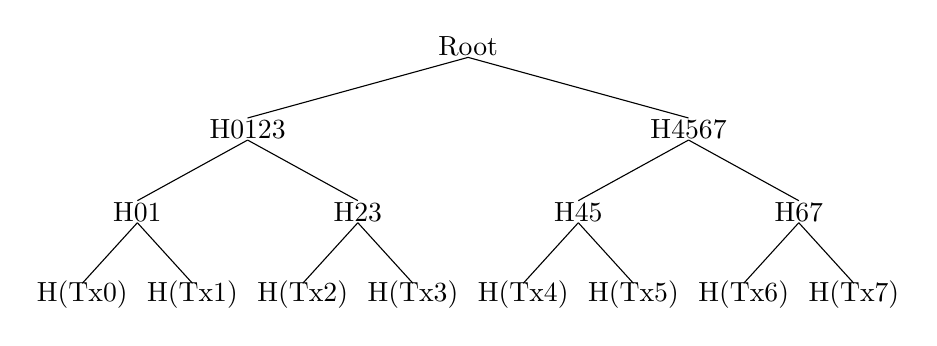
\begin{tikzpicture}[scale=0.7]
			% Leaf nodes
			\node at (0,0) {H(Tx0)};
			\node at (2,0) {H(Tx1)};
			\node at (4,0) {H(Tx2)};
			\node at (6,0) {H(Tx3)};
			\node at (8,0) {H(Tx4)};
			\node at (10,0) {H(Tx5)};
			\node at (12,0) {H(Tx6)};
			\node at (14,0) {H(Tx7)};

			% Level 1
			\node at (1,1.5) {H01};
			\node at (5,1.5) {H23};
			\node at (9,1.5) {H45};
			\node at (13,1.5) {H67};

			% Level 2
			\node at (3,3) {H0123};
			\node at (11,3) {H4567};

			% Root
			\node at (7,4.5) {Root};

			% Draw edges
			\draw (0,0.2) -- (1,1.3);
			\draw (2,0.2) -- (1,1.3);
			\draw (4,0.2) -- (5,1.3);
			\draw (6,0.2) -- (5,1.3);
			\draw (8,0.2) -- (9,1.3);
			\draw (10,0.2) -- (9,1.3);
			\draw (12,0.2) -- (13,1.3);
			\draw (14,0.2) -- (13,1.3);

			\draw (1,1.7) -- (3,2.8);
			\draw (5,1.7) -- (3,2.8);
			\draw (9,1.7) -- (11,2.8);
			\draw (13,1.7) -- (11,2.8);

			\draw (3,3.2) -- (7,4.3);
			\draw (11,3.2) -- (7,4.3);
		\end{tikzpicture}
	\end{center}
\end{frame}

\begin{frame}{Merkle trees in Bitcoin blocks}
	\begin{itemize}
		\item Each Bitcoin block header contains:
		      \begin{itemize}
			      \item Version number
			      \item Previous block hash
			      \item Merkle root of all transactions
			      \item Timestamp
			      \item Difficulty target
			      \item Nonce
		      \end{itemize}
		\item Block header is only 80 bytes.
		\item Merkle root represents all transactions in just 32 bytes.
	\end{itemize}
\end{frame}

\begin{frame}{Why use Merkle trees?}
	\begin{itemize}
		\item \textbf{Efficiency}: Verify transaction inclusion without full block.
		\item \textbf{Security}: Any change to transactions changes root.
		\item \textbf{Scalability}: Enables light clients (SPV wallets).
		\item \textbf{Privacy}: Can prove inclusion without revealing all transactions.
		\item \textbf{Storage}: Nodes can prune verified transactions, keep only headers.
	\end{itemize}
\end{frame}

\begin{frame}{Merkle proofs}
	\begin{itemize}
		\item To prove a transaction is in a block:
		      \begin{enumerate}
			      \item Provide the transaction.
			      \item Provide ``authentication path'' (sibling hashes).
			      \item Verifier recomputes hashes up to root.
			      \item Compare with known Merkle root.
		      \end{enumerate}
		\item Path length: $\log_2(n)$ for $n$ transactions.
		\item Example: 1000 transactions need only ~10 hashes.
	\end{itemize}
\end{frame}

\begin{frame}{Merkle proof example}
	\begin{itemize}
		\item Proving Tx2 is in the block:
	\end{itemize}
	\begin{center}
		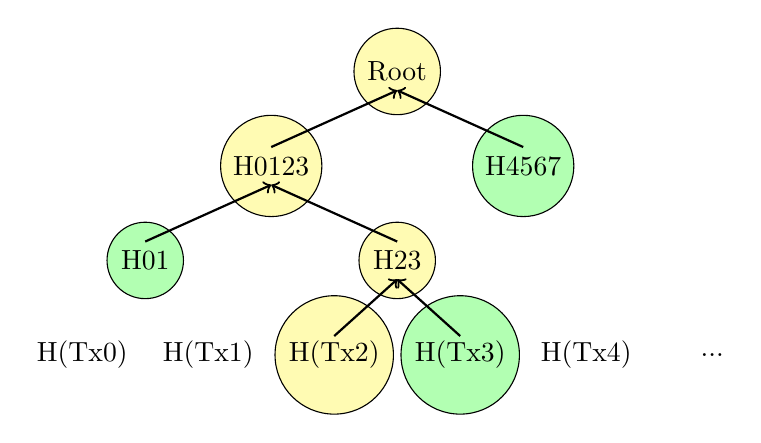
\begin{tikzpicture}[scale=0.8]
			% Highlight path
			\node[draw,circle,fill=yellow!30] at (4,0) {H(Tx2)};
			\node[draw,circle,fill=green!30] at (6,0) {H(Tx3)};
			\node[draw,circle,fill=yellow!30] at (5,1.5) {H23};
			\node[draw,circle,fill=green!30] at (1,1.5) {H01};
			\node[draw,circle,fill=yellow!30] at (3,3) {H0123};
			\node[draw,circle,fill=green!30] at (7,3) {H4567};
			\node[draw,circle,fill=yellow!30] at (5,4.5) {Root};

			% Other nodes
			\node at (0,0) {H(Tx0)};
			\node at (2,0) {H(Tx1)};
			\node at (8,0) {H(Tx4)};
			\node at (10,0) {...};

			% Draw relevant edges
			\draw[thick,->] (4,0.3) -- (5,1.2);
			\draw[thick,->] (6,0.3) -- (5,1.2);
			\draw[thick,->] (5,1.8) -- (3,2.7);
			\draw[thick,->] (1,1.8) -- (3,2.7);
			\draw[thick,->] (3,3.3) -- (5,4.2);
			\draw[thick,->] (7,3.3) -- (5,4.2);
		\end{tikzpicture}
	\end{center}
	\begin{itemize}
		\item Need: H(Tx2), H(Tx3), H01, H4567
	\end{itemize}
\end{frame}

\begin{frame}{Verification process}
	\begin{itemize}
		\item Given: Transaction Tx2 and proof [H(Tx3), H01, H4567]
		\item Verification steps:
		      \begin{enumerate}
			      \item Compute \func{hash}{Tx2}
			      \item Compute H23 = \func{hash}{\func{hash}{Tx2} \| H(Tx3)}
			      \item Compute H0123 = \func{hash}{H01 \| H23}
			      \item Compute Root = \func{hash}{H0123 \| H4567}
			      \item Check if computed root matches block header
		      \end{enumerate}
		\item Total data needed: ~100 bytes instead of entire block (~1MB)
	\end{itemize}
\end{frame}

\begin{frame}{SPV (Simplified Payment Verification)}
	\begin{itemize}
		\item Satoshi's solution for lightweight clients.
		\item SPV clients only download:
		      \begin{itemize}
			      \item Block headers (80 bytes each)
			      \item Merkle proofs for relevant transactions
		      \end{itemize}
		\item Storage requirement:
		      \begin{itemize}
			      \item Full node: ~500GB (all transactions)
			      \item SPV client: ~60MB (headers only)
		      \end{itemize}
		\item Trade-off: Trust that longest chain is valid.
	\end{itemize}
\end{frame}

\begin{frame}{Handling odd numbers of transactions}
	\begin{itemize}
		\item Merkle trees need even number of nodes at each level.
		\item Bitcoin's solution: Duplicate the last transaction if odd.
		\item Example with 5 transactions:
		      \begin{itemize}
			      \item Leaves: H(Tx0), H(Tx1), H(Tx2), H(Tx3), H(Tx4), H(Tx4)
			      \item Note: Tx4 hash is duplicated
		      \end{itemize}
		\item This ensures tree is always complete.
		\item Important: Duplicate the hash, not the transaction.
	\end{itemize}
\end{frame}

\begin{frame}{Security properties}
	\begin{itemize}
		\item \textbf{Tamper evidence}: Changing any transaction changes root.
		\item \textbf{Collision resistance}: Inherits from underlying hash function.
		\item \textbf{Second preimage resistance}: Can't find different transaction with same Merkle path.
		\item \textbf{Commitment}: Root commits to all transactions and their order.
	\end{itemize}
\end{frame}

\begin{frame}{Merkle tree attacks and defenses}
	\begin{itemize}
		\item \textbf{Potential attack}: Malicious miner includes invalid transaction.
		\item SPV clients can't detect without validating transaction.
		\item \textbf{Defense}: Economic incentives
		      \begin{itemize}
			      \item Invalid blocks rejected by full nodes.
			      \item Miner loses block reward.
			      \item Requires majority of miners to collude.
		      \end{itemize}
		\item \textbf{Best practice}: SPV clients should connect to multiple nodes.
	\end{itemize}
\end{frame}

\begin{frame}{Future improvements}
	\begin{itemize}
		\item \textbf{UTXO commitments}: Merkle tree of unspent outputs.
		\item \textbf{Fraud proofs}: Compact proofs of invalid transactions.
		\item \textbf{Merkle-sum trees}: Include transaction amounts in tree.
		\item \textbf{Alternative structures}:
		      \begin{itemize}
			      \item Verkle trees (more efficient proofs)
			      \item Sparse Merkle trees (better for state)
		      \end{itemize}
	\end{itemize}
\end{frame}

\begin{frame}{Merkle trees beyond Bitcoin}
	\begin{itemize}
		\item Used extensively in other cryptocurrencies:
		      \begin{itemize}
			      \item Ethereum: State tree, transaction tree, receipt tree
			      \item Certificate Transparency: Merkle tree of SSL certificates
			      \item Git: Similar structure for version control
			      \item IPFS: Content-addressed storage
		      \end{itemize}
		\item Key primitive for authenticated data structures.
		\item Enables efficient cryptographic commitments at scale.
	\end{itemize}
\end{frame}

\section{Bitcoin: More Intuitively}

\begin{frame}{Or, looking at it more intuitively...}
	\begin{columns}[c]
		\begin{column}{0.5\textwidth}
		\end{column}
		\begin{column}{0.5\textwidth}
		\end{column}
	\end{columns}
\end{frame}

\begin{frame}{Slides not complete and may contain errors}
	\begin{itemize}
		\item This slide deck is not finished, may contain errors, and is missing important material. Do not rely on it yet.
	\end{itemize}
\end{frame}

\begin{frame}[plain]
	\titlepage
\end{frame}
\end{document}
